\documentclass[aps,PRA,%
% jmp,
% bmf,
% sd,
% rsi,
 amsmath,amssymb,
%preprint,%
 %reprint,%
%author-year,%
%author-numerical,%
% Conference Proceedings,
%twocolumn,
singlecolumn,
notitlepage,superscriptaddress,groupedaddress]{revtex4}

\usepackage{setspace}


\usepackage{amsmath}
\usepackage[dvips]{graphicx}
\usepackage{epsfig}
\usepackage{tabularx}
\usepackage{color}
\usepackage[pdfpagemode=UseNone,colorlinks=true,linkcolor=blue,citecolor=blue]{hyperref}

\usepackage{soul}
\usepackage{gensymb}

\usepackage{makecell}

%\usepackage{subcaption}
%\usepackage{float}


\newcommand{\blu}[1]{{\color[rgb]{0,0,1}#1}}
\newcommand{\rosso}[1]{{\color[rgb]{1,0,0}#1}}
\newcommand{\verde}[1]{{\color[rgb]{0,0.7,0}#1}}
\newcommand{\viola}[1]{{\color[rgb]{1,0,1}#1}}

\newcommand{\red}[1]{{\color[rgb]{1,0,0}#1}}
\newcommand{\green}[1]{{\color[rgb]{0,0.7,0}#1}}

\renewcommand\Re{\operatorname{Re}}
\renewcommand\Im{\operatorname{Im}}
\newcommand{\fixme}[1]{\textcolor{red}{#1}}

\newcommand{\di}{i}  

\allowdisplaybreaks
\setcounter{MaxMatrixCols}{20}


\begin{document}



\title[]{Supplementary Material for: Strong coupling and dark modes in the motion of a pair of levitated nanoparticles}

\author{A. Pontin}
\email{antonio.pontin@cnr.it}
\affiliation{CNR-INO, largo Enrico Fermi 6, I-50125 Firenze, Italy}

\author{Q. Deplano}%
\affiliation{Dipartimento di Fisica e Astronomia, Università degli Studi di Firenze, via Sansone 1, I-50019 Sesto Fiorentino, Italy}%
\affiliation{INFN, Sezione di Firenze, via Sansone 1, I-50019 Sesto Fiorentino, Italy}

\author{A. Ranfagni}%
\affiliation{Dipartimento di Fisica e Astronomia, Università degli Studi di Firenze, via Sansone 1, I-50019 Sesto Fiorentino, Italy}%

\author{F. Marino}%
\affiliation{CNR-INO, largo Enrico Fermi 6, I-50125 Firenze, Italy}
\affiliation{INFN, Sezione di Firenze, via Sansone 1, I-50019 Sesto Fiorentino, Italy}


\author{F. Marin}
\email{marin@fi.infn.it}
\affiliation{CNR-INO, largo Enrico Fermi 6, I-50125 Firenze, Italy}
\affiliation{Dipartimento di Fisica e Astronomia, Università degli Studi di Firenze, via Sansone 1, I-50019 Sesto Fiorentino, Italy}%
\affiliation{INFN, Sezione di Firenze, via Sansone 1, I-50019 Sesto Fiorentino, Italy}
\affiliation{European Laboratory for Non-Linear Spectroscopy (LENS), Via Carrara 1, I-50019 Sesto Fiorentino, Italy}

%\begin{abstract}
%    Supplementary information for ``Title".
%\end{abstract}


\maketitle

\tableofcontents
%\doublespacing  



\section{Model}
As in standard description of coherent scattering (CS)~\cite{Vuletic2000Laser,novotny_CS_2019,Delic_CS_2019,toros2020Quantum,toros2021Coherent} we can write the total optical potential as $H_{\text{opt}}=- \mid \sqrt{\alpha_1} [\mathbf{E}_{1}(\mathbf{r}_1)+\mathbf{E}_{\text{cav}}(\mathbf{r}_1)]+\sqrt{\alpha_2}[\mathbf{E}_{2}(\mathbf{r}_2)+\mathbf{E}_{\text{cav}}(\mathbf{r}_2)]\mid^2/4$, where $\mathbf{r}_i$ and $\alpha_i$ are the two particles positions and their polarizability, $\mathbf{E}_i$ are the electric fields near the foci of the two trapping sites and $\mathbf{E}_\text{cav}$ is the intracavity field. As described in the main text, the second tweezer light (at $976$\,nm) is not resonant with the cavity so it does not participate in the CS interaction. The second particle interacts with the cavity mode through the scattered $1064$\,nm light from the first tweezer, which we write as $E_1(\mathbf{r}_2)=\zeta\,E_1(0)\,e^{i\varphi}$ where $\zeta$ and $\varphi$ account for the different amplitude and phase at the $976$\,nm focus. Without loss of generality, we will assume two identical particles to simplify the notation. We will also neglect the standard dispersive coupling which has been shown to be significantly smaller than the CS couplings. 



Before proceeding, it is useful to define the reference frame. We take the $1064$\,nm tweezer propagating along the \textit{z}-axis and with a polarization vector along the \textit{y}-axis. These directions are identified by the versors $\textbf{e}_z$ and $\textbf{e}_y$ respectively. The $976$\,nm tweezer is polarized along $\textbf{e}_x$. As a starting point for our definition, we consider a standard configuration where the cavity axis lies along $\textbf{e}_y$ and the cavity mode is polarized along $\textbf{e}_x$. In our setup, both tweezers polarizations are then rotated by an angle $\theta$ (see Fig. \ref{fig3sup}). However, it is convenient to keep the reference frame fixed on the tweezer and consider a rotated cavity frame. After rotation, the cavity mode is polarized along $\mathbf{e}_1$ and its axis lies along $\textbf{e}_2$. We also need to consider a deviation from orthogonality between the tweezer propagation direction and the cavity axis by a small angle $\theta_z$ to reflect an experimental imperfection. With this we can define $\mathbf{e}_1=\mathcal{R}(-\theta,\mathbf{e}_z)\mathcal{R}(-\theta_z,\mathbf{e}_x)\mathbf{e}_x$ and $\mathbf{e}_2=\mathcal{R}(-\theta,\mathbf{e}_z)\mathcal{R}(-\theta_z,\mathbf{e}_x)\mathbf{e}_y$ where $\mathcal{R}(\theta,\mathbf{e}_j)$ is a 3D rotation matrix around $\mathbf{e}_j$.




The optical Hamiltonian under consideration can then be written as

\begin{align}\label{eq1s} 
   H_{\text{opt}} & = \frac{\alpha}{4} \biggl[ \mid  \mathbf{E}_{1}(\mathbf{r}_1) \mid^2 + \mid \mathbf{E}_{2}(\mathbf{r}_2) \mid^2 \biggr. \nonumber\\
   &\biggl. + (\hat{a} E_d e^{-\di\mathbf{k}\cdot \mathbf{r}_1} f_{\text{c}} (\mathbf{r}_1) \mathbf{e}_1 \cdot \mathbf{e}_y  + \hat{a} \zeta E_d e^{-\di\mathbf{k}\cdot\mathbf{r}_2+\di\varphi} f_{\text{c}} (\mathbf{r}_2) \mathbf{e}_1 \cdot \mathbf{e}_y + h.c. )   \biggr].
\end{align}
Here, the first two terms are the 3D trapping potentials of the two particles, while the third term represents the coherent scattering interaction~\cite{Vuletic2000Laser,toros2021Coherent}. In Eq.~\ref{eq1s}, $E_d$ is the field driving the cavity from the first tweezer, i.e., $E_d\equiv E_1(0)$, $\mathbf{k}$ is the $1064$\,nm light wavevector, $\hat{a}$ is the cavity mode operator and $f_{\text{c}}(\mathbf{r}_i)$ is the cavity standing wave at the particles position which can be written as

\begin{equation}\label{eq2s}
    f_{\text{c}}(\mathbf{r}_i)=\epsilon_c^2 \cos(k\,\mathbf{e}_2\cdot \mathbf{r}_i+\phi_i)
\end{equation}

\noindent where we have neglected the Gaussian envelope of the cavity mode since $w_c\gg r_{12}$ (with $w_c$ the cavity waist). In Eq.~\ref{eq2s}, $k$ is the $1064$\,nm light wave number, $\phi_i$ identifies the particles position in the standing wave and we have included a normalization factor $\epsilon_c=\sqrt{2\hbar \omega_l/(\epsilon_0 V_c)}$ where $V_c=\pi w_c^2 L_c/4$ is the cavity mode volume, $L_c$ its length and $\omega_l$ is the laser angular frequency. If $\theta_z=0$ then $\phi_1=\phi_2$. In the case of a small, yet non-null $\theta_z$, since $\mathbf{r}_2=(x_2,y_2,z_2-r_{12})$, we can write  $\phi_2=\phi_1+k\,r_{12}\theta_z$. Considering that $r_{12}\simeq9\,\mu$m, even a small $\theta_z$ can have a significant impact on $\phi_2$.

Since the two particles are charged, the Coulomb potential must be considered as well. This is given by

\begin{equation}
    H_C=\frac{q_1 q_2}{4\pi\epsilon_0}\frac{1}{\sqrt{(r_{12}+z_1-z_2)^2+(y_1-y_2)^2+(x_1-x_2)^2}}
\end{equation}

\noindent where $q_i$ is the total charge on particle \emph{i}. We will show in Sec.~\ref{subscoulomb} that the dynamical Coulomb coupling provides only a minor contribution to the avoided crossings, however, one has to take into account the steady state shift along the \emph{z} direction as the power of  the second tweezer is varied to tune the eigenfrequencies of the system. To lowest order the steady state mean positions are given by

\begin{align}\label{eqs_steady}
    \bar{z}_1&= \frac{k_c r_{12}}{2 k_c (1+\omega_{z1}^2/\omega_{z2}^2)+r_{12}^3 m \omega_{z1}^{2}}\\
    \label{eqs_steady1}
    \bar{z}_2&= -\frac{k_c r_{12}}{2 k_c (1+\omega_{z2}^2/\omega_{z1}^2)+r_{12}^3 m \omega_{z2}^{2}}.
\end{align}

\noindent where we have defined $k_c=q_1q_2/(4\pi\epsilon_0)$ to simplify the notation. Although it is notoriously difficult to measure an absolute steady state shift, here only the change  related to the scan of $\omega_{z2}$ is relevant. To take it into account, we define $\Delta z$ to be the variation of the particles separation taking as a reference a given initial condition. The main consequence of $\Delta z$ is a variation of $\varphi$ while sweeping $\omega_{z2}$.

At this point, we can expand to second order the optical Hamiltonian and, moving to dimensionless units by normalizing the displacements to the respective zero point fluctuations ($zpf$), we obtain the following couplings between the cavity mode and the motional degrees of freedom

\begin{align}
    g_{x1}&\simeq -x_{1,zpf}\, g_0 \sin^2{\theta} \sin{\phi_1} \\
    g_{y1}&\simeq -y_{1,zpf}\, g_0 \cos{\theta}\sin{\theta} \sin{\phi_1} \\
    g_{z1}&\simeq -z_{1,zpf}\, g_0 \sin{\theta} (\di\cos{\phi_1}-\theta_z\sin{\phi_1})\\
    g_{x1y1}&\simeq - 2x_{1,zpf}\,y_{1,zpf}\, k\, g_0 \,\alpha_R \cos{\theta}\sin^2{\theta}\\
    g_{x2}&\simeq -x_{2,zpf}\, \zeta \,g_0 \,e^{\di(\varphi-k\,\Delta z)} \sin^2{\theta} \sin(\phi_1+k\,\theta_z r_{12}) \\
    g_{y2}&\simeq -y_{2,zpf}\, \zeta \,g_0 \, e^{\di(\varphi-k\,\Delta z)} \cos{\theta} \sin{\theta}\sin(\phi_1+k\,\theta_z r_{12}) \\
    g_{z2}&\simeq -z_{2,zpf}\, \zeta \,g_0 \, e^{\di(\varphi-k\,\Delta z)} \sin{\theta}[\di\cos(\phi_1+k\theta_z r_{12})-\theta_z\sin(\phi_1+k\theta_z  r_{12})]\\
    g_{x2y2}&\simeq - 2 x_{2,zpf}\,y_{2,zpf} \,\zeta\, k\, g_0 \cos \theta \cos(\phi_1+k\theta_z r_{12})\sin^2\theta\,[\alpha_R\cos(k \Delta z-\varphi)+\alpha_I \sin(k\Delta z-\varphi)]
\end{align}

\noindent where we have defined $g_0=\alpha\epsilon_ckE_d/(4\hbar)$. The steady-state intra-cavity field $\alpha_S=\alpha_R+\di \,\alpha_I$ is given by

\begin{equation}
    \alpha_S=\frac{g_0}{k}\frac{\cos \phi_1+\zeta e^{i (k \Delta z-\varphi)}\cos(\phi_1+k\theta_z r_{12})}{\Delta+ \di \,\kappa}\cos \theta.
\end{equation}

Since the experiment explores only the weak coupling limit, it is mathematically convenient to apply the rotating wave approximation for the mechanical degrees of freedom by introducing their creation and annihilation operators, and to adiabatically eliminate the cavity~\cite{Vijayan2024Cavity-mediated}. In this way one can reduce the dimensionality of the description and obtain an effective direct coupling between the mechanical oscillators. Furthermore, motion along the tweezers propagation direction (\emph{z}$_i$-axis) is largely decoupled from the motion in the transverse planes due to largely different oscillation frequencies. Thus, one can focus on the particles motion in their respective polarization planes. Finally, in our experimental configurations the particles are positioned close to a minimum of the intracavity field, therefore the direct couplings quantified by $g_{x1y1}$ and $g_{x2y2}$ have a negligible role and will be neglected in the following description.

The evolution equations for the cavity field $a$ and the mechanical operators $b_i$ can be written as 
\begin{eqnarray}
\dot{a} &=& \left(i\Delta-\frac{\kappa}{2}\right) a - i \Sigma_\alpha g_\alpha (b_\alpha + b^{\dagger}_\alpha) 
\label{eq_adot}\\
\dot{b}_\alpha &=& \left(-i\omega_\alpha-\frac{\gamma}{2}\right) b_\alpha -i (g_\alpha a^{\dagger}+g_\alpha^* a)
\label{eq_bdot}
\end{eqnarray}
where  the indexes vary though $(x_1,y_1,x_2,y_2)$, $\gamma$ is the mechanical damping rate and we are neglecting for the moment the input noise sources. In Eq. \ref{eq_bdot} the meaningful field terms are those rotating at the mechanical frequencies $\omega_\alpha$, while counter-rotating terms can be neglected. Therefore, from Eq. \ref{eq_adot} and its Hermitian conjugate we write 
\begin{eqnarray}
a &\simeq& \Sigma_\alpha\, \chi_c (\omega_\alpha)\, g_\alpha b_\alpha  
\label{eq_a}\\
a^{\dagger} &\simeq&  \Sigma_\alpha\, \chi_c^* (-\omega_\alpha) \,g_\alpha^* b_\alpha  
\label{eq_adag}
\end{eqnarray}
where $\chi_c (\omega) = 1/(\Delta + \omega +i \kappa/2)$ is the cavity susceptibility. Replacing Eqs. \ref{eq_a}-\ref{eq_adag} in Eq. \ref{eq_bdot} we obtain the cavity mediated coupling rates which, as reported in the main text, are given by
\begin{equation}\label{eq4s}
   G_{\alpha\beta}=\frac{g_\alpha g^*_{\beta}}{\Delta - \omega_\beta - \di\, \kappa/2} + \frac{g^*_\alpha g_{\beta}}{\Delta + \omega_\beta +\di\, \kappa/2}.
\end{equation}

The dynamics can then be described in compact form as

\begin{equation}\label{eqs_dyn}
    \frac{d}{dt}\mathbf{V}=-\di\,\mathbf{D}\mathbf{V}+\mathbf{V}_N
\end{equation}
\noindent where $\mathbf{V}=(b_{x1},b_{y1},b_{x2},b_{y2})$ is the variables vector, $\mathbf{V}_N$ the heating rate vector in which, in our experimental conditions, the only relevant contribution is thermal noise, and the dynamical matrix $\mathbf{D}$ is given by

\begin{equation}\label{eq3s}
    \mathbf{D}_{\alpha\beta}=\bigg[\omega_\alpha-\di\frac{\gamma}{2}\bigg]\delta_{\alpha\beta}+G_{\alpha\beta}.
\end{equation}

\subsection{Eigenvalues near an avoided crossing}\label{sec_eigen}
An eigenvalues analysis of the matrix $\mathbf{D}$ provides all the relevant information regarding the 2 particles dynamics. Even if fully analytical expressions can be calculated, these become cumbersome very quickly, and often a numerical approach is preferable. It is instructive to consider a single avoided crossing between two general modes of frequencies $\omega_1=\omega_0-\delta\omega$ and  $\omega_2=\omega_0+\delta\omega$ that are coupled according to Eq.~\ref{eq4s}. Without loss of generality, we neglect the gas damping $\gamma$.  The eigenvalues are then given by
\begin{equation}
    \lambda_{\pm}=\frac{1}{2}\bigg(2  \omega_0+G_{11}+G_{22}\pm\sqrt{4G_{12}G_{21}+(2\delta\omega+G_{22}-G_{11})^2}\bigg).
\end{equation}
Even in this case, expressions can be rather long so we report some meaningful approximated results. We take a purely conservative interaction with $g_2=\zeta g_1$, and we consider small variations of the frequencies around $\omega_0$, so that in $G_{ij}$ we set $\omega=\omega_1=\omega_2$ and by defining 
\begin{equation}
    G_{00}= g_1^2 \left[ \frac{1}{\Delta-\omega_0+\di\kappa/2}+\frac{1}{\Delta+\omega_0-\di\kappa/2} \right]
\end{equation}
we can write $G_{11}=G_{00}$, $G_{12}=G_{21}=\zeta G_{00}$, and $G_{22}=\zeta^2 G_{00}$.
Moreover, the experimental parameters allow us to expand the eigenvalues assuming a large detuning limit, i.e., $\mid\Delta\mid\gg\kappa,\omega_i$, therefore we are also giving simplified expressions valid in this limit. 

As a first analysis, we search the minimal eigenfrequencies separation. Far from the crossing (i.e., for $|\delta\omega| \gg 2 g^2/|\Delta|$) the two eigenfrequencies are
\begin{align}
    \Omega_1&\,\simeq\,\omega_0-\delta\omega+\mathrm{Re}[G_{11}] \,\simeq\,\omega_0-\delta\omega+\frac{2g_1^2}{\Delta}\bigg( 1-\frac{\kappa^2/4-\omega_0^2}{\Delta^2}\bigg)\\
   \Omega_2&\,\simeq\,\omega_0+\delta\omega+\mathrm{Re}[G_{22}] \,\simeq\, \omega_0+\delta\omega+\frac{2\zeta^2 g_1^2}{\Delta}\bigg( 1-\frac{\kappa^2/4-\omega_0^2}{\Delta^2}\bigg)
\end{align}
\noindent which shows the cavity-induced frequency shift of the two modes. The crossing, defined by the minimal splitting between eigenfrequencies, occurs at
\begin{equation}
    \delta\omega=\frac{1}{2}\left(1-\zeta^2\right) \mathrm{Re}[G_{00}] = \frac{(1-\zeta^2)g_1^2}{\Delta} \bigg( 1-\frac{\kappa^2/4-\omega_0^2}{\Delta^2}\bigg)
\end{equation}
\noindent where the eigenvalues are given by
\begin{align}\label{eqs_eigen1}
    \lambda_\pm& 
    =\omega_0+\frac{1}{2}(\zeta\mp1)^2 \,G_{00}
    =\omega_0+\frac{(\zeta\mp1)^2g_1^2}{\Delta}\bigg(1-\frac{\kappa^2/4-\omega_0^2}{\Delta^2}\bigg)+\di \frac{(\zeta\mp1)^2g_1^2\kappa\omega_0}{\Delta^3}\\
    &=\Omega\mp \frac{2\zeta g_1^2}{\Delta}\bigg(1-\frac{\kappa^2/4-\omega_0^2}{\Delta^2}\bigg)+\di \frac{(\zeta\mp1)^2g_1^2\kappa\omega_0}{\Delta^3}
\end{align}
\noindent with a corresponding frequency splitting of $\delta_{12}=-\frac{4\zeta g_1^2}{\Delta}(1-\frac{\kappa^2/4-\omega_0^2}{\Delta^2})$.  The values reported in the main text correspond to a lower order expansion. 

As a second analysis, we consider $\delta\omega=0$, i.e., the bare frequencies crossing. The two eigenvalues are now given by
\begin{align}
    \lambda_+&=\omega_0\\
    \lambda_-&=
    \omega_0+(\zeta^2+1)\,G_{00}
    =\omega_0+\frac{2(\zeta^2+1)g_1^2}{\Delta}\bigg(1-\frac{\kappa^2/4-\omega_0^2}{\Delta^3}\bigg)-\di\frac{2(\zeta^2+1)g_1^2\kappa\omega_0}{\Delta^3}
\end{align}
\noindent which shows an unmodified upper branch and a downshifted and broadened  lower branch (for red detunings).

\subsection{Dark mode formation}
As in Sec.~\ref{sec_eigen}, we consider a simplified scenario with two coupled modes. The objective is to evaluate the cavity mode and show that, when the conditions for the dark mode formation are met, the upper branch decouples from it and would not appear in the cavity field spectrum. As before, we consider $g_2=\zeta g_1$ and, since we are interested in a region close to the avoided crossing, we approximate the couplings in Eq.~\ref{eq4s} by considering $\omega_{1}\simeq\omega_{2}\simeq\omega_0$ allowing us to rewrite Eq.~\ref{eq3s} as
\begin{equation}
    \mathbf{D}=\begin{pmatrix}
        \omega_\alpha&0\\
        0&\omega_\beta
    \end{pmatrix}+
    G_{00}\begin{pmatrix}
        1 & \zeta\\
        \zeta&\zeta^2
    \end{pmatrix} \, .
\end{equation}

\noindent Solving Eq.~\ref{eqs_dyn} in the Fourier domain one finds
\begin{equation}
    \mathbf{V}=(\di\omega\,\mathbf{I}+\di\mathbf{D})^{-1}\mathbf{V}_N=\mathbf{B}\mathbf{V}_N
\end{equation}
\noindent where $\mathbf{V}_N=(v_{1in},\, v_{2in})^{T}$, with $v_{1in}$ and $v_{2in}$ being the two modes heating rates. The matrix $\mathbf{B}$ is given by
\begin{equation}\label{eq_sol}
    \mathbf{B}=\frac{1}{\Delta_D}\begin{pmatrix}
        \di(\omega_2-\omega)+\zeta^2G_{00}&-\zeta G_{00}\\
        -\zeta G_{00}&\di(\omega_1-\omega)+G_{00}
    \end{pmatrix}=\frac{G_{00}}{\Delta_D}\begin{pmatrix}
        \zeta^2&-\zeta\\
        -\zeta&1
    \end{pmatrix}.
\end{equation}
Here, $\Delta_D=\mathrm{Det}[\di\omega\,\mathbf{I}+\di\mathbf{D}]$ and in the last step we have set $\omega=\omega_1=\omega_2$. 
Using Eqs.~\ref{eq_a} and \ref{eq_sol} we find
\begin{equation}
    a=\frac{\chi_c(\omega)\,g_1 G_{00}}{\Delta_D}\bigg[ \left( \zeta^2 v_{1in}-\zeta v_{2in}\right)+\zeta \left( -\zeta v_{1in}+v_{2in} \right)   \bigg]=0
\end{equation}
\noindent which shows that the dark mode always forms where the bare frequencies cross regardless of the value of $\zeta$.

\subsection{Coulomb coupling}\label{subscoulomb}
The Coulomb interaction provides a dynamical coupling between the particles degrees of freedom along with the steady state displacement of Eqs.~\ref{eqs_steady}-\ref{eqs_steady1}. This can be calculated by expanding to second order $H_C$ leading to an additional spring constant for each direction given by
\begin{align}
       k_z&=\frac{2 k_c}{r_{12}^3}\\
    k_{x,y}&=-\frac{k_c}{r_{12}^3}.
\end{align}
Focusing on the motion on the polarization planes, this contribution is included in the model by adding to the dynamical matrix $\mathbf{D}$ in Eq.~\ref{eqs_dyn} the following matrix
\begin{equation}
\mathbf{C}= g_c\begin{pmatrix}
\omega_{x1}^{-1} & 0 & (\omega_{x1}\omega_{x2})^{-1/2} & 0 \\
0 & \omega_{y1}^{-1} & 0 & (\omega_{y1}\omega_{y2})^{-1/2} \\
(\omega_{x1}\omega_{x2})^{-1/2} & 0 & \omega_{x2}^{-1} & 0 \\
0 & (\omega_{y1}\omega_{y2})^{-1/2} & 0 & \omega_{y2}^{-1}
\end{pmatrix}
\end{equation}

\noindent where $g_c=-k_c/2mr_{12}^3\equiv \frac{k_{x,y}}{2m}$. Two considerations can be made. First, it only contributes to the avoided crossing visible at $P_{\mathrm{tw2}}\simeq0.33$\,W in Fig.~3 of the main text, with a coupling that can be estimated to be $g_x\approx g_y\approx2\pi120$\,Hz thus representing only a small correction. Second, the cavity mediated interaction of Eq.~\ref{eq3s} has a periodic dependence on $\varphi$ with a period of $\pi$, however, the simultaneous presence of the Coulomb interaction breaks this periodicity which then becomes $2\pi$. 



\section{Eigenfrequencies fitting}
As stated in the main text we model the experiment with nominal particle and cavity parameters. The latter are all measured independently while the former are consistent with previously reported measurements by our group~\cite{Ranfagni2021Two-dimensional}. This leaves four parameters to be estimated: the deviation from orthogonality between the cavity axis and the tweezers propagation direction ($\theta_z$), the position of the first particle ($1064$\,nm tweezer) in the cavity standing wave $\phi_1$, the fields ratio $\zeta$ and their relative phase $\varphi$.

For the evaluation of the angle $\theta_z$ we adopt a dedicated approach. Firstly, it is measured independently  by translating a single particle along the \emph{z}-axis through the cavity mode cross-section~\cite{Ranfagni2021Vectorial}.  The estimated value is $\mid\theta_z\mid=(1\pm0.5)\degree$. Notice that the method used does not allow to ascertain the sign of $\theta_z$, however, the final result does not depend on it, so we assume a positive sign. Despite the fact that $\theta_z$ is quite small, it is still sufficient to have a large impact since in the current experiment we cannot independently control the position of the two particles. For example, if we consider the first particle to be at a cavity node, i.e., $\phi_1=\pi/2$, for the second one we would have $\phi_2=\phi_1+k r_{12}\theta_z\simeq2.5$, corresponding to a shift of $160$\,nm along $z$. The particle is therefore more than halfway to the adjacent cavity antinode. This makes it clear that the direct measurement of $\theta_z$ is not sufficiently accurate, and its value needs to be varied within the experimental uncertainty.

The last point before discussing the fitting procedure concerns the reference value for $\Delta z$. This has been set by choosing the reference as the equilibrium position when the power on the second tweezer is $P_{\mathrm{tw2}}=280$\,mW, yielding $\omega_{z2}/2\pi\simeq23.3$\,kHz. Given the range of $P_{\mathrm{tw2}}$ exploited in the experiment, $\Delta z$ explores $\sim300$\,nm which correspond to an overall scan  of $\varphi$   by roughly   $110\degree$. Thus, this represents a non-negligible effect.

For the parameters fitting we proceed as follows. First, we initially fix $\theta_z$ and create three 2D maps $\mathcal{F}_i(\phi_1,\varphi)$  of the three splittings $\delta_{\alpha\beta}$, with $i=(x_1x_2,y_1y_2,x_1y_2)$, for each value of the fields ratio $\zeta$ in the range 0.28-0.45 with a resolution of 0.017. To generate the map, the eigenfrequencies of the dynamical matrix $\mathbf{D}$, including the Coulomb term, are calculated varying the power of the second tweezer $P_{\mathrm{tw2}}$. The three splittings are obtained as minimal differences between eigenfrequencies. We then use a least square method to extract the optimal values of $\phi_1$ and $\varphi$, that is we minimize
\begin{equation}\label{eqs_lsq}
    \mathcal{L}=\sum_i \bigg(\frac{\mathcal{F}_i-\delta_i}{\sigma_i}\bigg)^2=\sum_i\mathcal{L}_i
\end{equation}
\noindent where $\delta_i$ are the measured splitting values and $\sigma_i$ their standard deviation. Considering $\mathcal{L}$ as a function of $\zeta$ allows to select the optimal fields ratio. The procedure is then repeated for different values of $\theta_z$ within the experimental uncertainty.
\begin{figure}[ht]
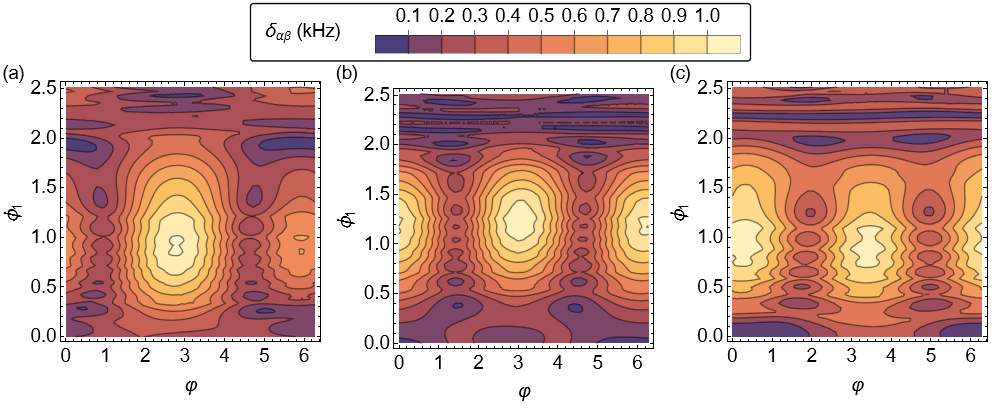
\includegraphics[width=\textwidth]{fig1_sup_splt_map.png}
\caption{Analytical 2D maps of the three splittings $\delta_{x1x2}$, $\delta_{y1y2}$ and $\delta_{x1y2}$ shown in a), b) and c) respectively as a function of the fields relative phase $\varphi$ and the position in the cavity standing wave $\phi_1$.
}\label{fig1sup}
\end{figure}
An example of the maps is shown in Fig.~\ref{fig1sup} for $\theta_z=1\degree$ and $\zeta=0.28$  which correspond to the initial estimate. It is immediate to see that $\delta_{y1x2}$ and $\delta_{x1y2}$, in Fig.~\ref{fig1sup}~b) and Fig.~\ref{fig1sup}~c) respectively,  approximately retain a periodicity of $\pi$ in $\varphi$, while $\delta_{x1x2}$ in Fig.~\ref{fig1sup}~a) does not. This is expected since $\delta_{x1x2}$ is the only one significantly affected by the Coulomb coupling 

At the end of the procedure the extracted parameters are $\theta_z=(0.75\pm0.13)\degree$,  a fields ratio $\zeta=0.35\pm0.015$ with a relative phase $\varphi=(172\pm3)\degree$ and a position along the standing wave of $\phi_1=1.225\pm0.015$.  This corresponds to the first particle being $\sim58$\,nm away from the node, and the second one $\sim 59$\,nm away on the opposite side.  %Notice that if $\theta_z$ is negative the position of the two particles with respect to the node would swap but nothing else would change.
%\rosso{DA DOVE VIENE L'ERRORE SUI PARAMETRI?}

To demonstrate the solidity of the procedure we show in Fig.~\ref{fig2sup}~b) the individual contributions $\mathcal{L}_i$, around the global minimum of $\mathcal{L}$, as a function of the map parameters $(\phi_1,\varphi)$. For each contribution we plot a region close to the local minimum $min(\mathbf{L}_i)$ with an upper clipping equal to $1/\sigma_i$. The global minimum occurs at the intersection of all three regions. In Fig.~\ref{fig2sup}~a) and Fig.~\ref{fig2sup}~c) we show the same plots with identical boundaries for the adjacent values of $\zeta$. It is clear that in neither case there is an intersection of all three regions.

\begin{figure}[ht]
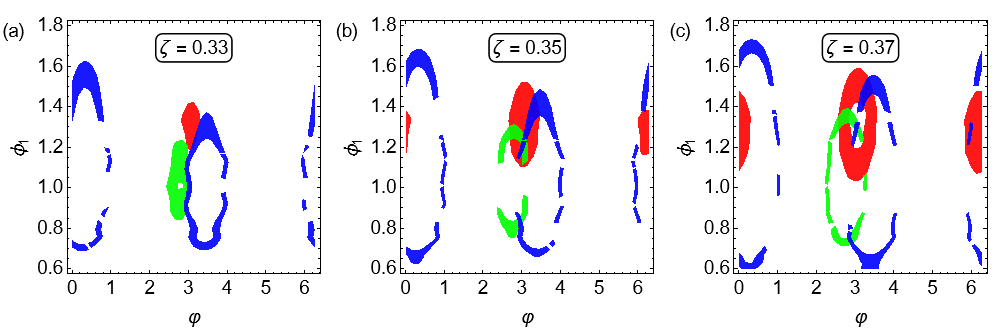
\includegraphics[width=\textwidth]{fig2_sup_chisqr_V2.png}
\caption{Region plot for the individual contributions to $\mathcal{L}$ near the respective local minima. For all panels $\theta_z=0.75\degree$. The upper clipping is kept constant and equal to $1/\sigma_i$. The regions in red, blue and green correspond respectively to $\delta_{y1,x2}$, $\delta_{x1,y2}$ and $\delta_{x1,x2}$. The three panels correspond to different values of the fields ratio $\zeta$ with a) $\zeta=0.33$, b) $\zeta=0.35$,  c) $\zeta=0.37$. The second value yields the global minimum of $\mathcal{L}$, and indeed only in panel b) there is an intersection of all of the three plotted regions. 
}\label{fig2sup}
\end{figure}


\section{Analysis of additional contributions to the dynamics.}

\subsection{Overlap of the two trapping potentials}
Here we are interested in evaluating the perturbation on one particle due to the optical field used to trap the other. Since the two trapping positions are along the propagation direction, there will be both a gradient and a scattering force acting on a particle as a result of the off-focus optical field trapping the other. This modifies the total potential and influences the equilibrium position of the two particles. Importantly, to evaluate these contributions we do not require precise knowledge of the electric fields at the focus since the particles separation is much larger than the typical waist at the two foci. Thus, we can use the nominal Gaussian beam parameters that can be calculated for the aspheric lens doublet used to generate the optical tweezer. As stated in the main text, the two light fields are delivered through a polarization maintaining (PM) fiber which is first collimated, with a focal length $f=18.4$\,mm, and then rifocused by a second asphere, $f=3.1$\,mm. The fiber numerical aperture has been measured to be $NA=0.098\pm0.003$ which gives a waist of $w_{976}=0.53\pm0.02$ at $976$\,nm and $w_{1064}=0.58\pm0.02$ at $1064$\,nm. With these, the off-focus fields can be calculated with a standard Gaussian beam description.

The effect of the gradient force $F_{gr}$ can be calculated using the potential $H_{tw}=-\alpha \mid  \mathbf{E}(\mathbf{r})\mid^2/4$ while the radiation pressure force is given by $F_{rp}=P_{sc}/c$, where $P_{sc}$ is the total scattered power. Since we are interested in these forces in the linear part of the Gaussian beam expansion it is convenient to write approximate expressions. After some algebra one finds
\begin{align}\label{eqs_forces}
    F_{gr,j}&=\frac{2\alpha P_{tw,i}}{\pi c\epsilon_0}\frac{z_{R,i}^2}{w_i^2 z_{0,i}^3}\bigg( 1+\frac{3 z_i}{z_{0,i}} \bigg)=F_{gr0}+k_{gr} z_i\\
    \label{eqs_forces1}
    F_{rp,j}&=\frac{2P_{tw,i}\sigma_{sc,i}}{\pi c}\frac{z_{R,i}^2}{w_i^2z_{0,i}^2}\bigg(1+\frac{2z_i}{z_{0,i}}\bigg)=F_{rp0}+k_{rp}  z_i  
\end{align}
\noindent where the index refers to the two wavelengths, $z_{R,i}$ is the Rayleigh range, $\sigma_{sc,i}=\alpha^2k_i^4/(6\pi\epsilon_0^2)$ the Rayleigh cross section and $\alpha=\epsilon_0\chi V_s$ is the particle polarizability with $V_s$ the particle volume and $\chi$ its susceptibility. Given the experimental geometry, we have $z_{0,976}=r_{12}$ and $z_{0,1064}=-r_{12}$. These forces have to be compared with those resulting from the main optical potential. To do this, we use the experimental trap frequencies, thus we avoid the necessity of knowing the electric field at the foci. The steady state position is then given by $z_j=(F_{gr,i}+F_{rp,i})/m\omega_{z,j}^2$ and the modified trap frequencies are given by $\omega_{zf,j}=\sqrt{\omega_{z,j}^2-(k_{gr}+k_{rp})/m}$. When inserting in Eqs.~\ref{eqs_forces}-\ref{eqs_forces1} the parameters for the current experiment, we find that the steady state shift is larger for the particle in the $976$\,nm trap since the forces sum up. However, the estimated shift is of the order of $\sim100$\,nm, and it is just a few tens of nanometers for the particle in the $1064$\,nm trap. Thus, in both cases it remains negligible. As for the frequency shift, it is dominated by the softening gradient force contribution which for both particles remains smaller than $\sim200$\,Hz. 


\subsection{Contribution to recoil heating}
Since the particles are illuminated by both beams there will be an additional recoil heating term. In general, the recoil heating rate for the center of mass motion is given by~\cite{Seberson2020Distribution}
\begin{equation}\label{eqs_recoil}
    \Gamma_{0}=\Lambda\frac{\omega_l}{\Omega}\frac{P_{sc}}{mc^2}
\end{equation}
\noindent where $c$ is the speed of light, $\omega_l=kc$, $P_{sc}$ is the total scattered power and the coefficient $\Lambda=(\frac{2}{10},\frac{1}{10},\frac{7}{10})$ takes into account the dipole pattern of the scattered light, $\Omega=(\omega_{x},\omega_{y},\omega_{z})$ are the different trap frequencies.  The scatter power can be written as $P_{sc}=\sigma_{sc}\epsilon_0c |E_0|^2/2$ where $E_0$ is the field at the trap center. This allows us to directly calculate the recoil $\Gamma_d$ at distance $d=r_{12}$, since we have $|E_{d}|=\zeta |E_0|$. In particular, the heating rate ratio is $\Gamma_{d}/\Gamma_0=\zeta^2=0.12$, assuming identical frequencies. Such a small ratio simply reflects the fact that $\Gamma$ depends on the intensity, while the coupling to the cavity depends on the field.

However, the total recoil per particle depends on the different wavelengths and, more importantly, on the orthogonal polarizations of the two trapping fields. For simplicity, we will assume identical parameters for the foci of the two traps, but the following can be generalized for different geometries. Thus, for the particle in the $1064$\,nm trap there  will be the usual recoil term plus the contribution due to the off focus $976$\,nm field
\begin{equation}\label{eqs_rqcoil1}
\begin{split}
    \Gamma_{1,0}&= \Lambda_1 \Xi_1 |E_1|^2/\Omega_1     \\
    \Gamma_{2,d}&=\Lambda_2 \Xi_2 \zeta^2 |E_2|^2/\Omega_1.  
\end{split}
\end{equation}
Here, the indexes $i=(1,2)$ identify the $1064$ and  $976$ traps respectively, the fields are considered at the center of the respective trap, $\Lambda_1=(\frac{2}{10},\frac{1}{10},\frac{7}{10})$, $\Lambda_2=(\frac{1}{10},\frac{2}{10},\frac{7}{10})$ and $\Xi_i=\epsilon_0 k_i \sigma_{sc,i}$. Similarly, for the particle in the $976$\,nm trap we have
\begin{equation}
    \begin{split}\label{eqs_recoil2}
    \Gamma_{2,0}&= \Lambda_2 \Xi_2 |E_2|^2/\Omega_2     \\
    \Gamma_{1,d}&=\Lambda_1 \Xi_1 \zeta^2 |E_1|^2/\Omega_2.  
\end{split}
\end{equation}
Thus, using Eqs.~\ref{eqs_rqcoil1}-\ref{eqs_recoil2} we can quantify the increase of recoil heating with the ratios
\begin{equation}
\begin{split}
    \frac{\Gamma_{2,d}}{\Gamma_{1,0}}&=\bigg(\frac{1}{2},2,1\bigg)\bigg(\frac{k_2}{k_1}\bigg)^5\zeta^2 (1+P_0 \Delta P) \\
     \frac{\Gamma_{1,d}}{\Gamma_{2,0}}&=\bigg(2,\frac{1}{2},1\bigg)\bigg(\frac{k_1}{k_2}\bigg)^5\zeta^2 (1+P_0 \Delta P)^{-1}
\end{split}
\end{equation}
\noindent where we set $P_{tw1}=P_0$ and $P_{tw2}=P_0+\Delta P$. Assuming identical powers, $\Delta P=0$,  we have $\Gamma_{2,d}/\Gamma_{1,0}=(0.04,0.16,0.08)$ and $\Gamma_{1,d}/\Gamma_{2,0}=(0.38,0.09,0.19)$ where the larger contribution is due to the polarization orientation.
    
\subsection{Optical binding}
Optical binding arises from the interference between the trapping fields and the scattered light. Thus, 
at each particle position there are two interfering terms, one for each wavelength. It is possible to show that, to the leading order, the coupling for the motion along \emph{z} vanishes and one is left with coupling terms $\propto x_1 x_2$ and $\propto y_1 y_2$ without mixed terms.

Along the $x$ and $y$ directions one can define an equivalent spring constant for each wavelength. For the particle in the $1064$\,nm trap we have
\begin{equation}\label{eqs_k1}
    k_{OB,i}=-\frac{\alpha^2k_i^3}{4\pi\epsilon_0 \,c\,d^2}\sqrt{I_{i,0}I_{i,d}}\,\,[1+(z_R/d)^2]^{-\frac{1}{2}},
\end{equation}
\noindent the index $i=(1,2)$ identify the $1064$\,nm and  $976$\,nm wavelenghts respectively.  On the other end, for the particle in the $976$\,nm trap we have
\begin{equation}\label{eqs_k2}
    k_{OB,i}=-\frac{\alpha^2k_i^3}{4\pi\epsilon_0 \,c\,d^2}\sqrt{I_{i,0}I_{i,d}}\,\sin\Phi_i
\end{equation}
\noindent where $\Phi_i=2k_i d-\arctan\frac{d}{z_R}$.  Eqs.~\ref{eqs_k1}-\ref{eqs_k2} are valid for both $x$ and $y$ directions and allow to calculate the coupling rates. Considering the parameters of the current experiment the estimated coupling is of the order of $g_{OB}/2\pi\sim1$\,Hz for all four terms  in Eqs.~\ref{eqs_k1}-\ref{eqs_k2} and is thus negligible. A detailed calculation for  Eqs.~\ref{eqs_k1}-\ref{eqs_k2} can be found in the supplemental document of Ref.~\cite{Deplano2024Coulomb}.

\section{Experimental setup}
The optical layout of the experiment is shown in Fig.~\ref{fig3sup}.  A first Nd:YAG at $1064$\,nm is used to lock a high finesse optical cavity by implementing a PDH lock scheme. A second Nd:YAG laser at $1064$\,nm and a laser diode at $976$\,nm are used to create a bichromatic tweezer creating two trapping sites separated by  $r_{12}=9\pm1\,\mu$m. The particles are positioned at the center of the cavity with a 3 axes translational stages. The two Nd:YAG lasers are phase locked with a frequency offset corresponding to one cavity free spectral range (FSR). The experimental setup is described in details elsewhere, additional information can be found in Refs.~\cite{Ranfagni2021Vectorial,Ranfagni2021Two-dimensional}. The loading method is described in Ref.~\cite{Calamai2021Transfer} while the bichromatic tweezer and the particles charge characterization can be found in Ref.~\cite{Deplano2024Coulomb}.

\begin{figure}%[ht]
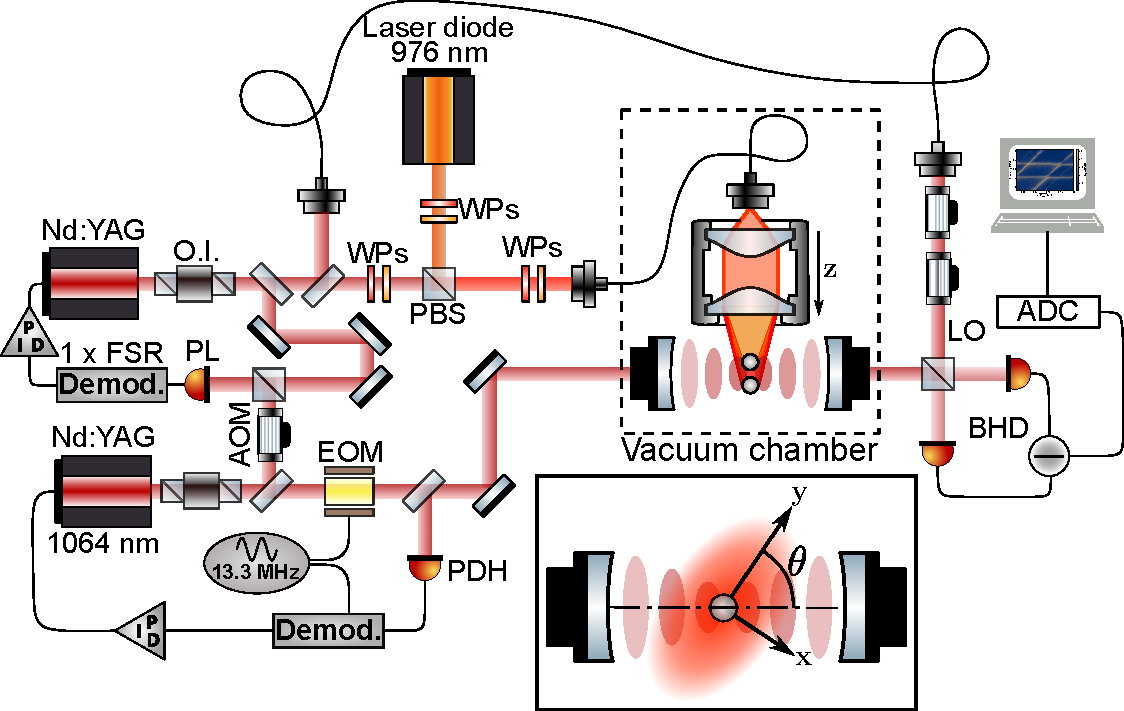
\includegraphics[width=12.0cm]{fig1_v1.pdf}
\caption{Optical layout. O.I: optic isolator, WP: wave plate, PBS: polarizing beam-splitter, AOM: acousto-optic modulator, EOM: resonant electro-optic modulator, FSR: free-spectral range, PDH: Pound-Drever-Hall detection, LO: local oscillator, BDH: balanced heterodyne detection, ADC: analog-to-digital converter.  
}\label{fig3sup}
\end{figure}


\bibliographystyle{nicebib}
\bibliography{main_bib}


\end{document} 